\section{Durchführung}
\label{sec:Durchführung}

\subsection{Versuchsaufbau}
Der Pupmstand ist wie in Abbildung \ref{fig:Aufbau} aufgebaut. Hier ist es wichtig
möglichst genau zu arbeiten, da sonst Fehler durch Lecks an Gummis und Flanschen
entstehen.
\begin{figure}
  \begin{subfigure}[c]{0.5\textwidth}
    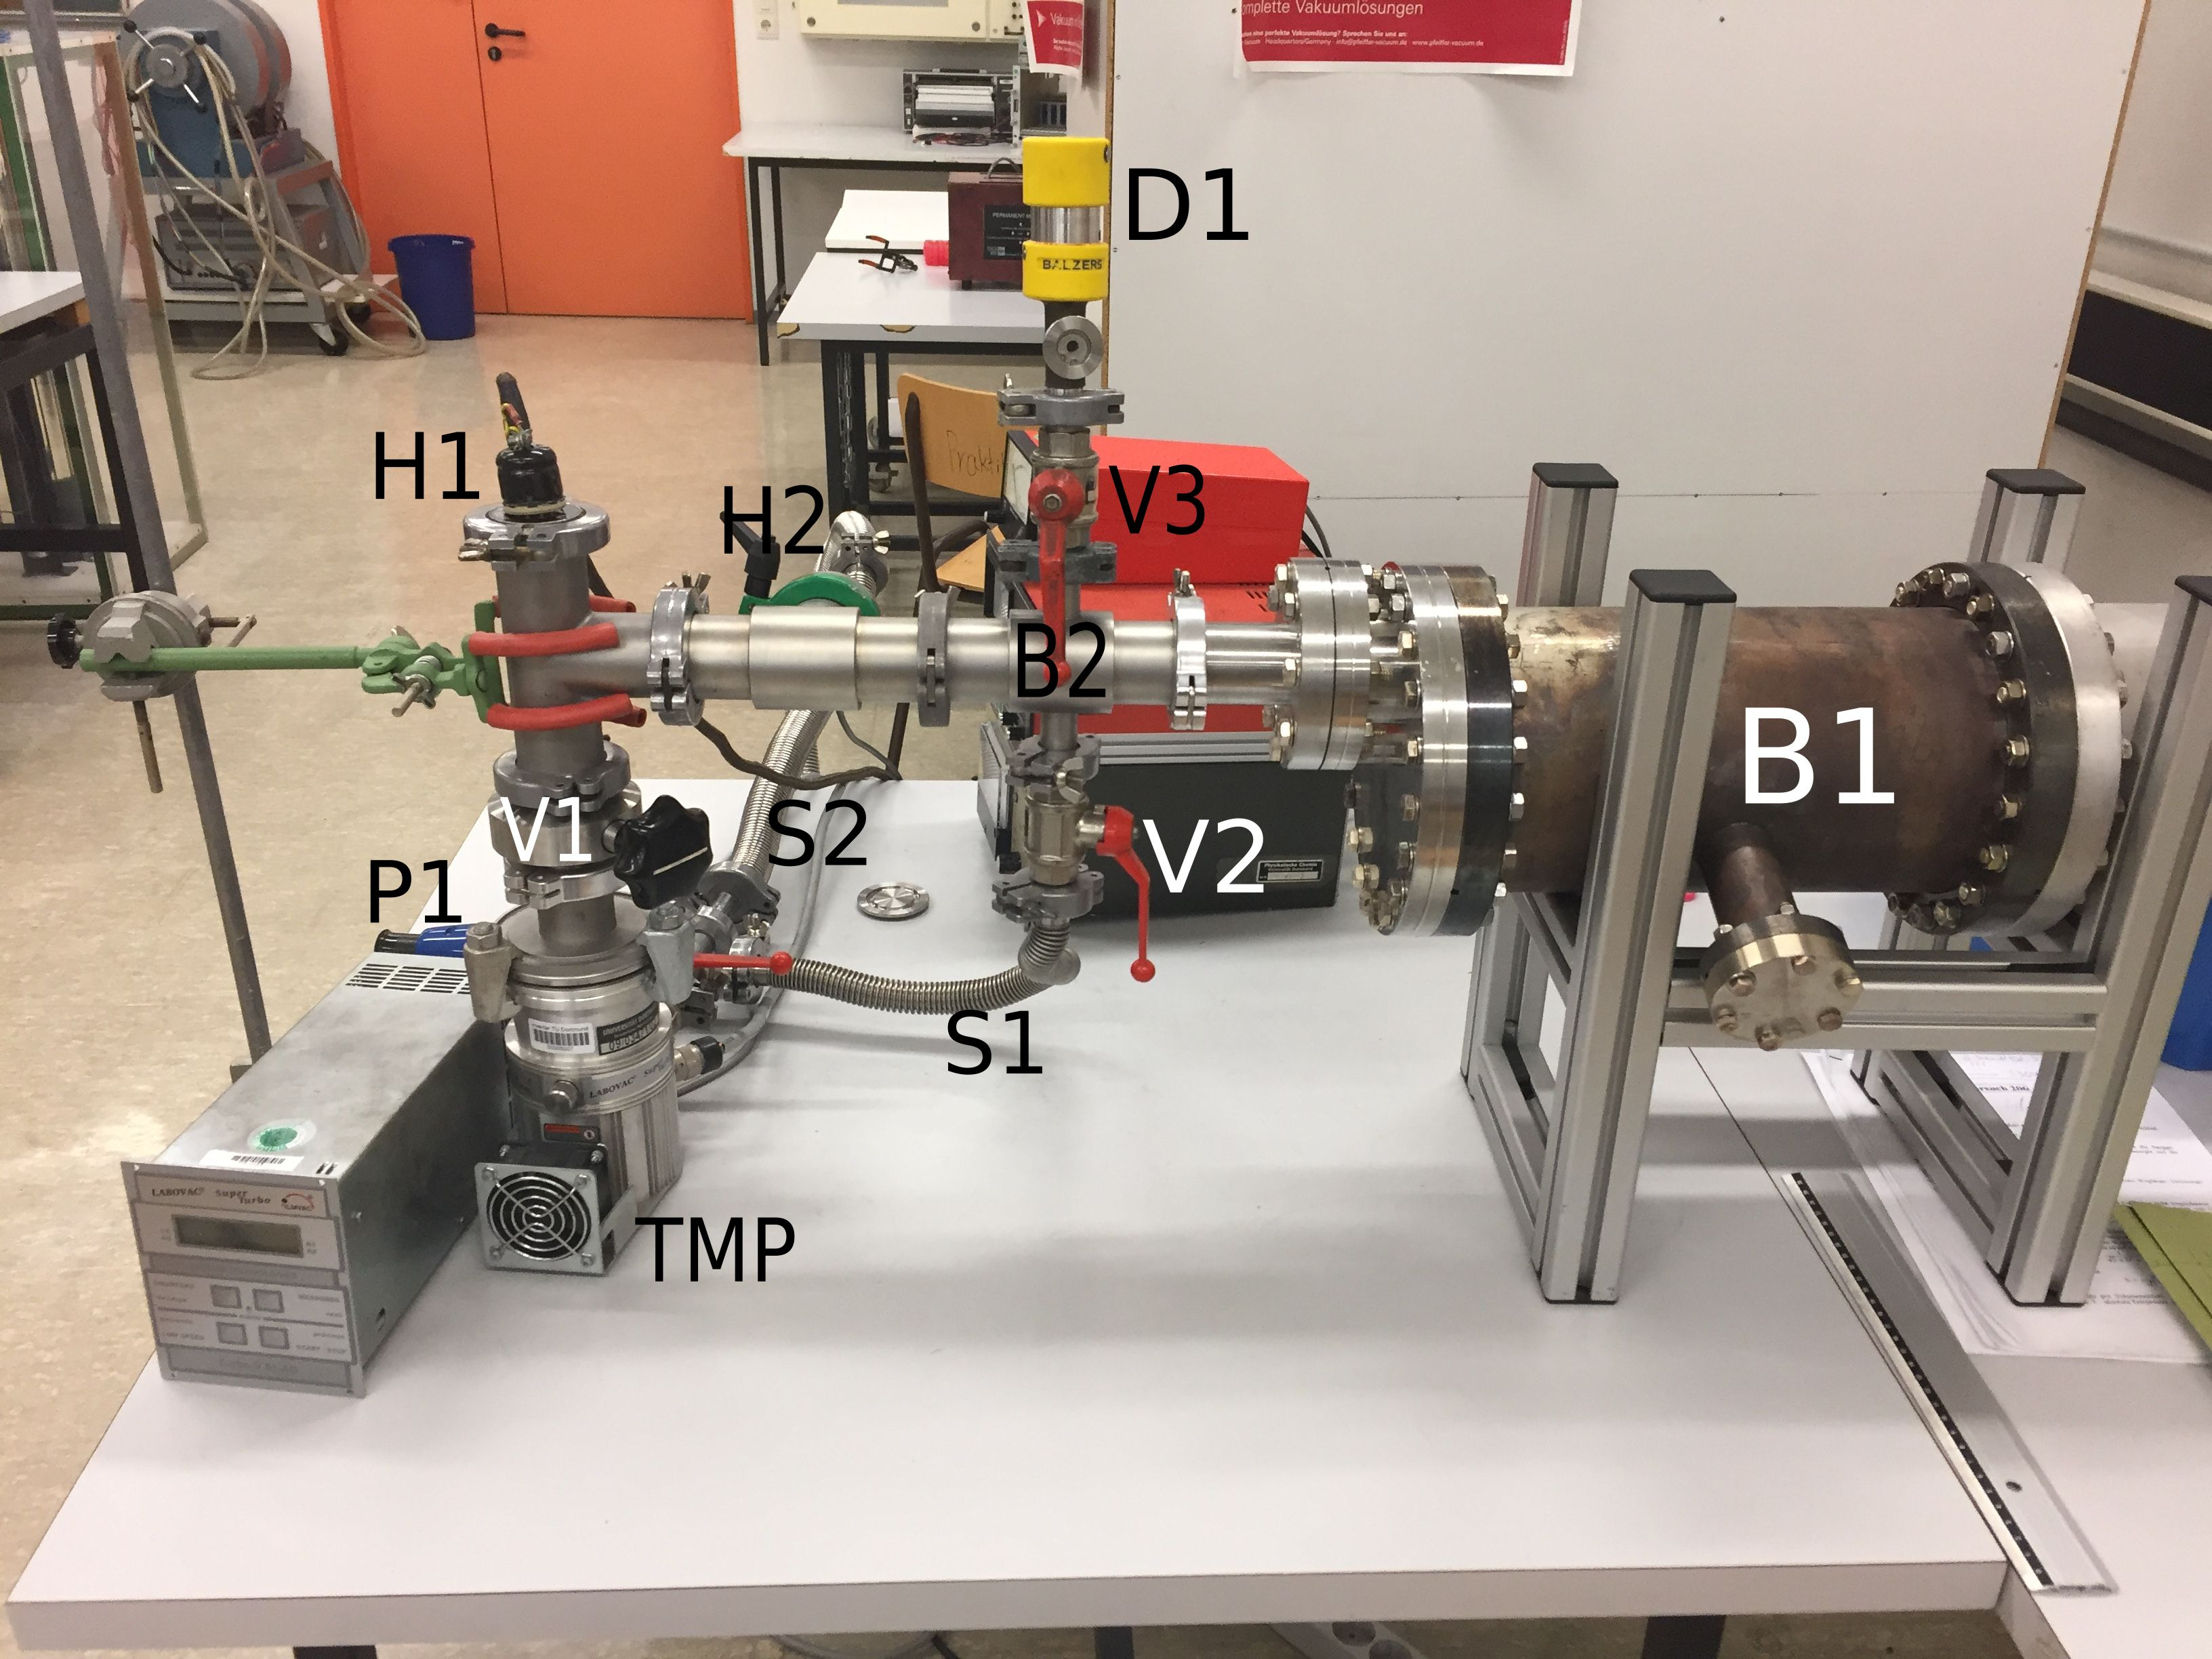
\includegraphics[width=\textwidth]{IMG_6888.JPG}
  \end{subfigure}
  \begin{subfigure}[c]{0.5\textwidth}
    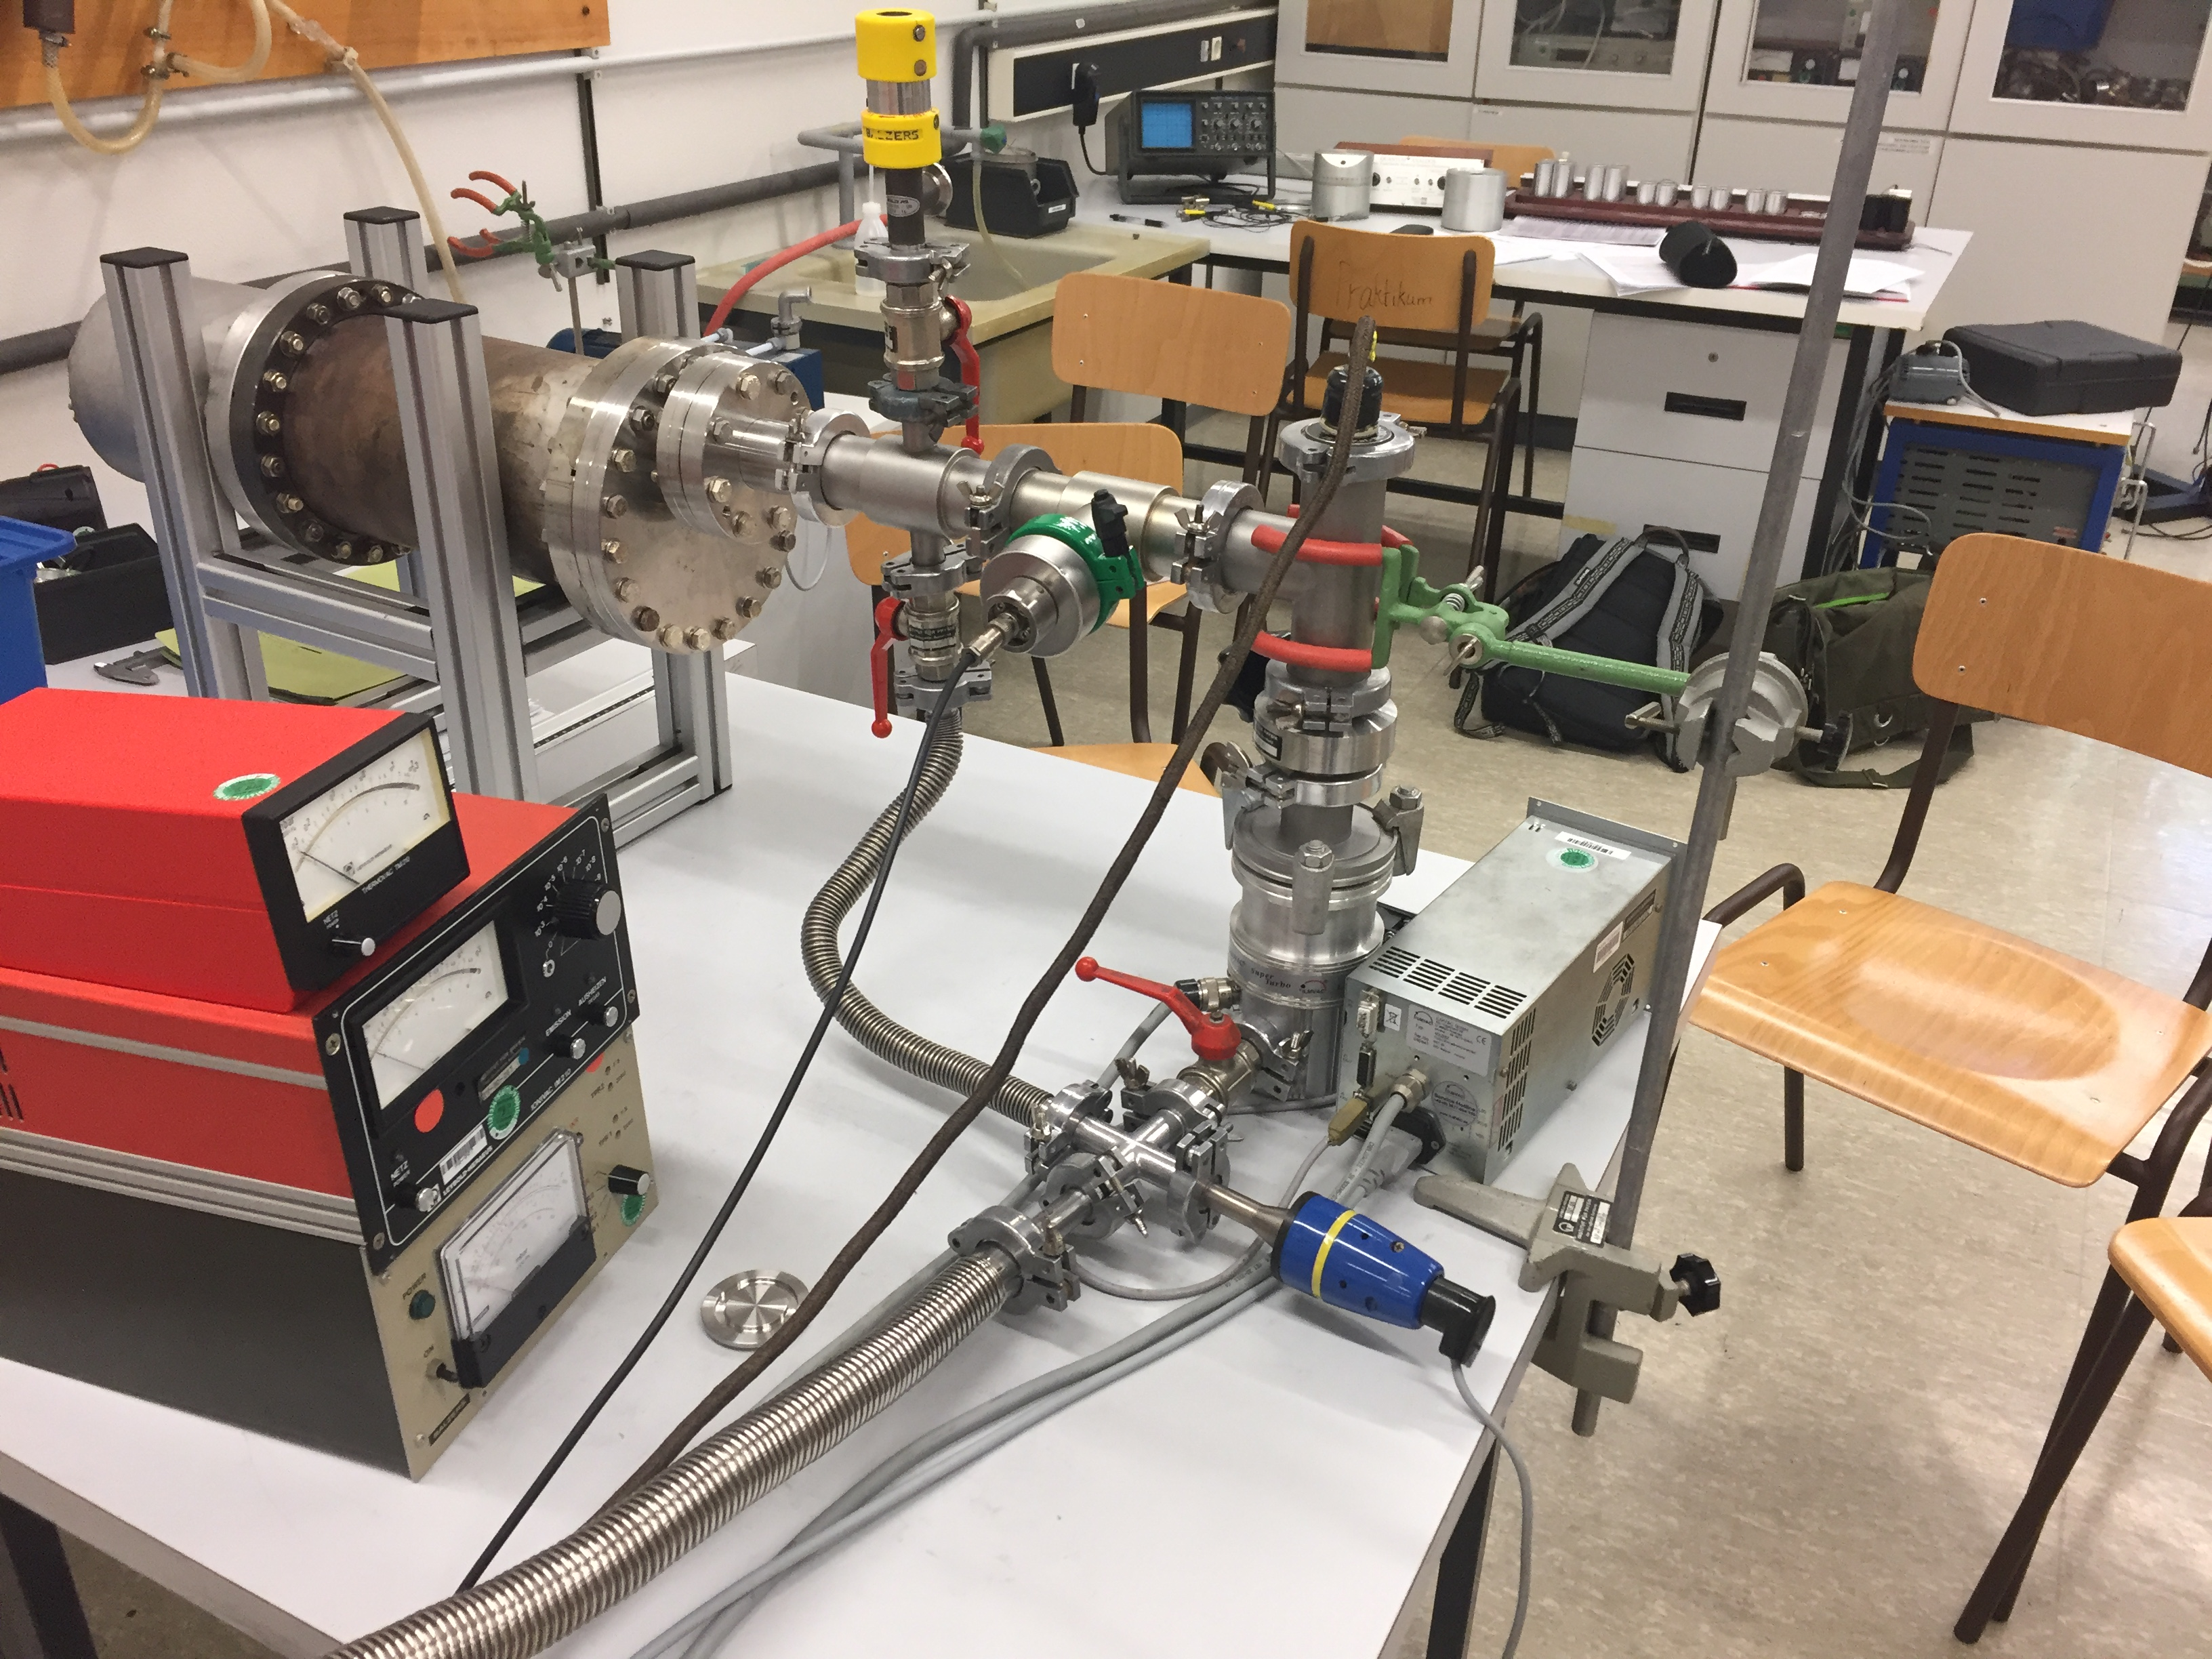
\includegraphics[width=\textwidth]{IMG_6889.JPG}
  \end{subfigure}
  \caption{Aufbau des Pumpstandes und Beschriftung der Einzelteile.}
  \label{fig:Aufbau}
\end{figure}

Dabei wurden diejenigen Teile verwendet, die aus Tabelle \ref{tab:Teile} bzw. Abbildung
\ref{fig:Teile} zu entnehmen sind.

\begin{figure}
  \centering
  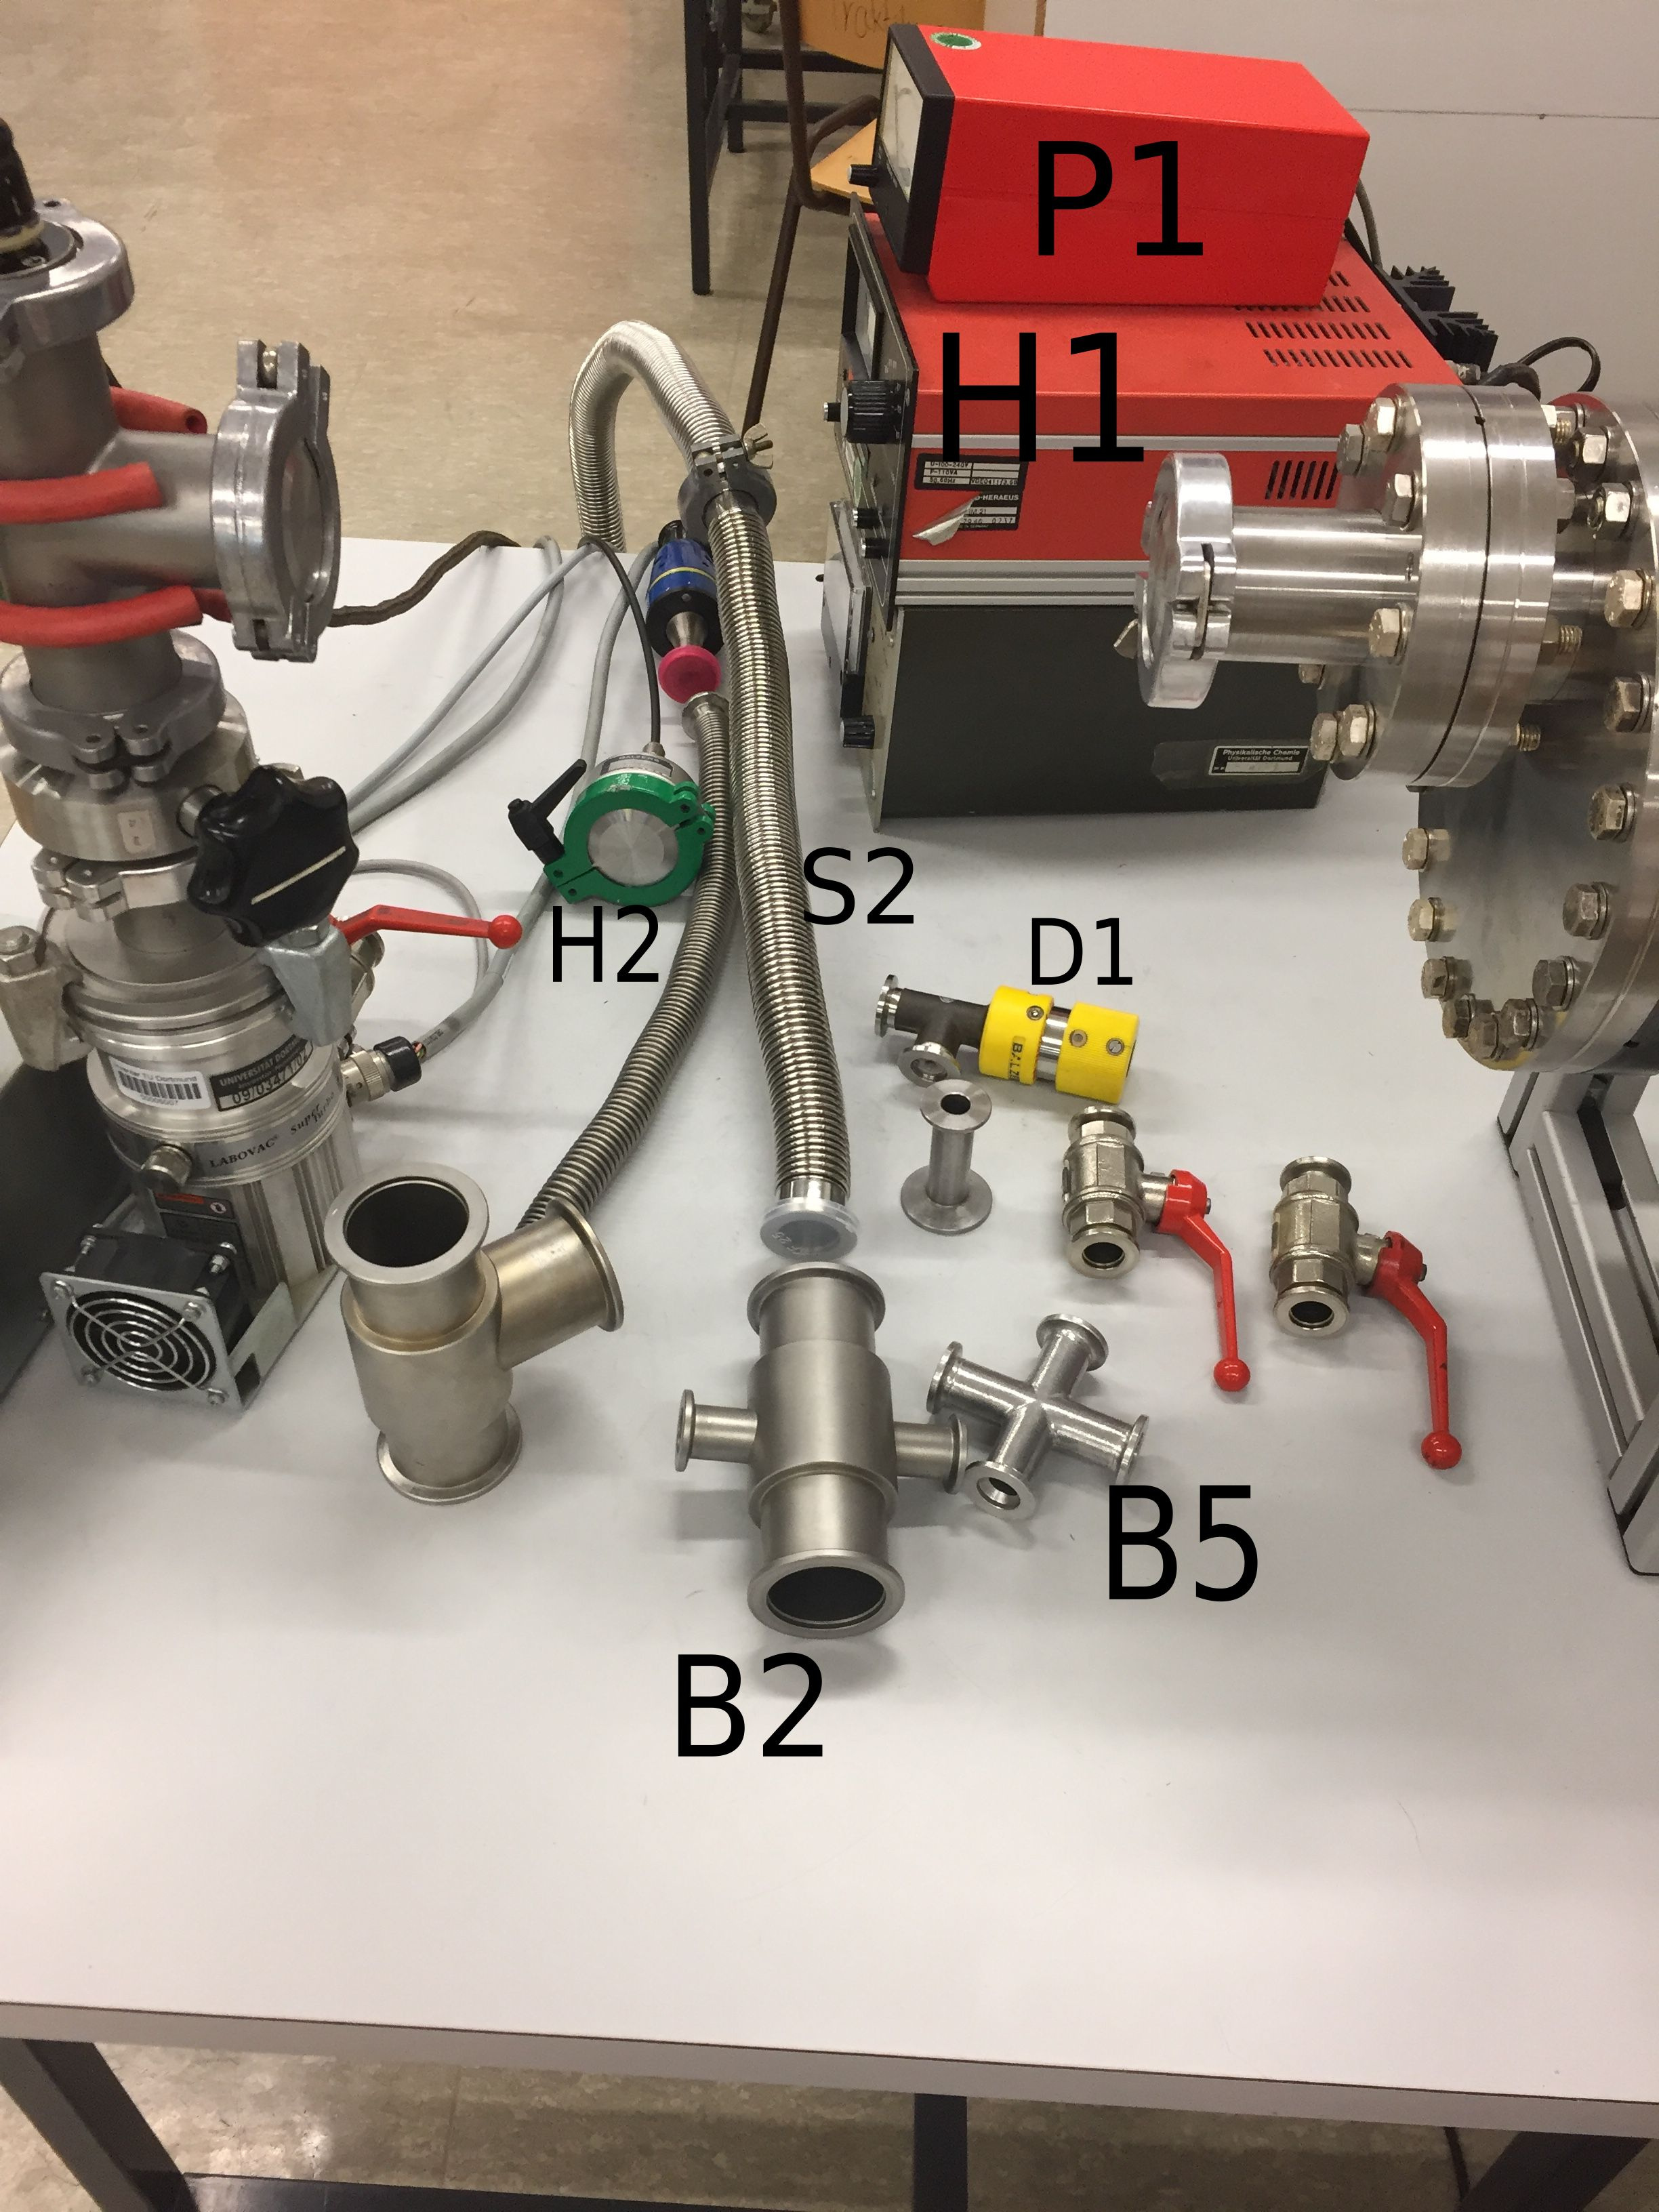
\includegraphics[width=0.4\textwidth]{IMG_6891.JPG}
  \caption{Verwendete Teile zum Aufbau des Pumpstandes.}
  \label{fig:Teile}
\end{figure}

\begin{table}
  \caption{Verwendete Bauteile zum Aufbau des zur Messung verwendeten Pumpstandes \cite{anleitung}.}
  \label{tab:Teile}
  \begin{tabular}{c c | c c}
    \toprule
    Abkürzung & Bezeichnung/Name & Abkürzung & Bezeichnung/Name \\
    \midrule
    S1 & Schlauch 1 & D1 & Dosierventil 1 \\
    S2 & Schlauch 2 & P1 & analoges Pirani Druckmessgerät \\
    B1 & großer Rezipient & B2 & Bauteil \\
    B3 & Bauteil & B4 & Bauteil \\
    B5 & Bauteil & B6 & Bauteil \\
    V1 & Klappenventil & V2 & Kugelventil 2 \\
    V3 & Kugelventil 3 & V4 & Kugelventil 4 \\
  \end{tabular}
\end{table}
Zuerst wird der Pumpstand mit der Drehschieberpumpe evakuiert. Nach ungefähr 10$\,$min
stellt sich ein Druck von $\SI{5e-2}{\milli\bar}$ ein und die TMP kann hinzugeschaltet
werden.
Jetzt kann das Glühkathoden Vakuummeter eingeschaltet werden. Nun kann der Rezipient
ca. 10$\,$min der Rezipient mit dem Heißluftföhn erhitzt werden. Das führt dazu,
dass Wasserablagerungen im Rezipienten verdampfen und so die Desorptionsrate abnimmt.
Wird ein Enddruck zwischen $\SIrange{2e-5}{8e-5}{\milli\bar}$ erreicht, so gilt der
Aufbau als dicht und es kann mit den Messungen begonnen werden.

\subsection{Messungen}
\subsection{Evakuierungskurve der Drehschieberpumpe}
Zuerst wird die TMP durch das schließen von V1 und V5 abschiebert und V2 geöffnet.
Bei laufender Drehschieberpumpe werden nun dir Belüftungsventile D1 und V3 geöffnet
um den Rezipienten aus Atmosphärendruck zu bringen. Daraufhin werden die Belüftungsventile
wieeder geschlossen und der Druckabfll gegen die zeit aufgenommen. Diese Messung wird
5-mal durchgeführt.
\subsection{Leckratenmessung der Drehschieberpumpe}
Bei laufender Drehschieberpumpe wird durch D1 ein Gleichgewichtsdruck $p_\text{G}$
im Rezipienten erzeugt und nach abschiebern von V4 der Druckanstieg mit der Zeit
aufgenommen. Dies find für die Gleichgewichtsdrücke $p_\text{G}$ = {$\SI{0.1}{\milli\bar}$,
$\SI{0.4}{\milli\bar}$, $\SI{0.8}{\milli\bar}$, $\SI{1.0}{\milli\bar}$} jeweils 3-mal
durchgeführt.

Bevor nun die Messungen an der TMP durchgeführt werden können, muss diese wieder
hinzugeschaltet werden. Dazu wird V1 und V5 geöffnet und V2 geschlossen. Wenn der
Druck durch die Drehschieberpumpe unter $\SI{5e-5}{\milli\bar}$ gefallen ist, kann
die TMP eingeschaltet werden.
\subsection{Evakuierungsmessung der Turbomolukularpumpe}
Bei laufender TMp wrd durch D1 ein Druck von $\SI{5e-3}{\milli\bar}$ eingestellt
und nun D1 und V3 möglichst zeitgleich geschlossen. Der auftretende Druckabfall
wird mit der Zeit aufgenommen. Diese Messung wird analog zu der bei der Drehschieberpumpe
5-mal widerholt.
\subsection{Leckratenmessung der Turbomolukuralpumpe}
Analog zur Leckratenmessung  der Drehschieberpumpe wird auch hier mit Hilfe des Nadelentils
D1 ein Gleichgewichtsdruck $p_\text{G}$ eingestellt und dann V1 geschlossen. Daraufhin
kann der Druckanstieg über das Glühkathoden Vakuummeter und die Zeit aufgenommen werden.
Diese Messung wird bei $p_\text{G}$ = ${\SI{5e-5}{\milli\bar}, \SI{10e-5}{\milli\bar},
\SI{150e-5}{\milli\bar}, \SI{20e-5}{\milli\bar}}$ jeweils 3-mal durchgeführt.

\subsection{Volumenbestimmung}
Da sich das Volumen des Rezipienten aufgrund von geschlossenen Ventilen und Verbindungsstücken
bei jeder Messreihe ein wenig ändert muss das Gesamtvolumen bestimmt werden. Dazu werden
die verwendeten Teile nach dem Abbau des Pumpstandes mit Lineal und Schieblehre ausgemessen
und bei der Volumenberechnung miteinbezogen.
